\section{STAKEHOLDER REQUIREMENTS} % http://dilbert.com/strip/2006-01-29
The stakeholders for AndrOS are:

\begin{enumerate}
	\item The course instructor
  \item The student (Tristan Andrus)
  \item Totally Legit, Inc., a potential customer.
\end{enumerate}


\subsection{Stakeholders User Stories}
The primary stakeholders needs are described below.

%As a course instructor I need equipment in the control systems lab that provides students with a useful hands-on experience.
\bigskip
  
In order to be useful the lab equipment used must not be mysterious (or overly 'black box').
\bigskip
  
Students need to see the inputs and outputs of the system and understand that they can replicate similar systems in their careers.
\bigskip
		
The power amplifier module must be constructed of a technology that is familiar to both mechanical and electrical/computer engineering students at a late-junior year level.  In order to meet this familiarity requirement the design is constrained to use a power operational amplifier.
\bigskip
		
The power amplifier needs to be a unity voltage gain non-inverting buffer. 
\bigskip

The power amplifier must provide a minimum continuous output current of 8 amps.
\bigskip

The input impedance of the power amplifier must be greater than or equal to 10 kilohms.
\bigskip
		
The largest time constant of the power amplifier must be less than 0.001 seconds.
\bigskip


%%\subsubsection{The course instructors}
%%\begin{enumerate}
%%  \item As a course instructor, I want the student to develop a project that is challenging but doable. 
%%  \item I also want the project to consist of at least 200 hours of technical effort.
%%\end{enumerate}



\subsubsection{The student}
\begin{enumerate}
  \item As a student, I want the project to be an exciting demonstration of my engineering prowess.
  \item However, I also want to specify a project that is achievable with my limited time and money
\end{enumerate}


\subsubsection{Totally Legit, Inc, a Potential Customer}
\begin{enumerate}
  \item As a totally real and not made up company, Totally Legit, Inc. wants a low-overhead system that can read what is on flash drives without booting into Windows or some other easily-compromised software system.
  \item We also want an operating system to use as a springboard for some of our embedded systems.
\end{enumerate}

\begin{figure}[h]
  \centering
  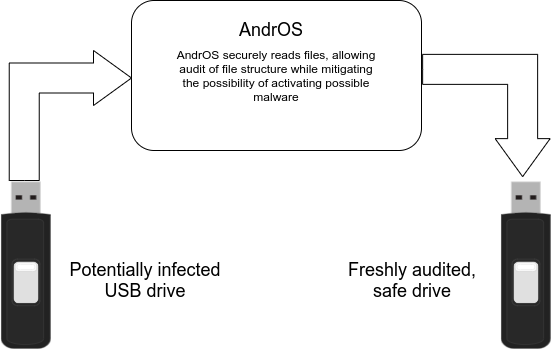
\includegraphics[width=\textwidth]{andrus-totally-legit-diagram.png}
  \caption{Block diagram of Total Legit, Inc.'s use for AndrOS.}
\end{figure}
